\documentclass[border=10pt]{standalone}
\usepackage{tikz}
\usetikzlibrary{arrows.meta, calc, shapes}

\begin{document}
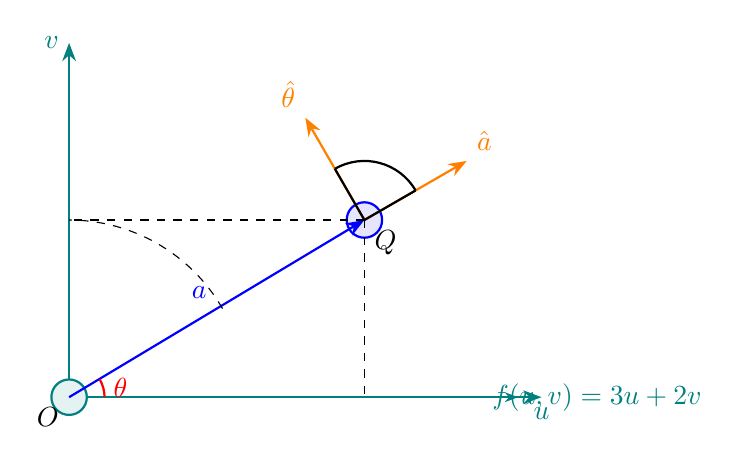
\begin{tikzpicture}[scale=1.5, >=Stealth]

% Axes
\draw[thick, teal, ->] (0,0) -- (4,0) node[below] {$u$};
\draw[thick, teal, ->] (0,0) -- (0,3) node[left] {$v$};

% Origin O
\draw[fill=teal!10, draw=teal, thick] (0,0) circle (0.15) node[below left] {$O$};

% Point Q
\coordinate (Q) at (2.5,1.5);
\draw[fill=blue!10, draw=blue, thick] (Q) circle (0.15) node[below right] {$Q$};

% Vector a
\draw[thick, blue, ->] (0,0) -- (Q) node[midway, above left] {$a$};

% Angle theta at origin
\draw[thick, red] (0.3,0) arc (0:30:0.3) node[midway, right] {$\theta$};

% Unit vectors at Q
\draw[thick, orange, ->] (Q) -- ++(30:1) node[above right] {$\hat{a}$};
\draw[thick, orange, ->] (Q) -- ++(120:1) node[above left] {$\hat{\theta}$};

% Dashed lines for coordinates
\draw[dashed] (Q) -- (Q |- 0,0);
\draw[dashed] (Q) -- (Q -| 0,0);

% Circular arc centered at O passing through Q
\draw[dashed] (0,0) ++(30:1.5) arc (30:90:1.5);

% Function label
\node[teal, right] at (3.5,0) {$f(u,v) = 3u + 2v$};
\draw[teal, ->] (3.2,0) -- (3.8,0);

% Angle between unit vectors at Q
\draw[thick] (Q) ++(30:0.5) arc (30:120:0.5);
\draw[thick] (Q) ++(30:0.5) -- (Q) ++(30:0.5) ++(0.1,0);
\draw[thick] (Q) ++(120:0.5) -- (Q) ++(120:0.5) ++(0.1,0);

\end{tikzpicture}
\end{document}